\chapter{繁殖与环境}\label{ch:g8:reproduction-and-environment}

为什么蛙群的合唱始于五月而非十一月？为什么
丰年的山毛榉会让林地长满\omterm{prop:g2:from-seed-to-plant:cycle}{幼苗}，而一个
寒冷潮湿的六月却让来年春天的池塘几乎不见幼蛙？上一章
讲了下一代产生的机制，本章则
把它放回真实世界：繁殖有时间安排、有物质供应，
——也受\omterm{def:g6:exploring-our-environment:components}{环境}的限制。

\section{时机由季节决定}

\begin{proposition}[繁殖遵循丰饶的时令]\label{prop:g8:reproduction-and-environment:timing}
\omterm{def:g5:biodiversity:species}{物种}安排繁殖时间，使\emph{幼体}
出生时恰逢\omterm{def:g6:exploring-our-environment:conditions}{条件}适宜、食物充足
（见\cref{prop:g6:life-through-seasons:conditions}）：
\begin{itemize}
  \item 蓝山雀的产卵时间恰好使雏鸟孵化于春季
        \omterm{ex:g2:animals-grow-up:butterfly}{毛毛虫}高峰期（\cref{ex:g3:food-chains:three}
        中的橡树\omterm{def:g3:food-chains:chain}{食物链}，精确到天）；
  \item 青蛙在变暖的池塘中产卵，
        让\omterm{ex:g2:animals-grow-up:frog}{蝌蚪}在入冬前有一整个夏天生长；
  \item \omterm{def:g1:plants-around-us:plant}{植物}的开花期与\omterm{def:g5:flower-to-fruit:steps}{传粉}者的活跃季节相配，
        \omterm{def:g2:from-seed-to-plant:seed}{种子}成熟则与传播的时节相配，
        （见\cref{pb:g6:life-through-seasons:1}）；
  \item 雄鹿秋季的鸣叫，
        决定下一个\emph{春季}的出生，妊娠期已计算在内。
\end{itemize}
启动这一机制的线索，
正是\omterm{def:g6:exploring-our-environment:components}{环境}自身的信号：首先是日照渐长，其次是温暖和降雨。
\end{proposition}
\admitted

\begin{omfigure}
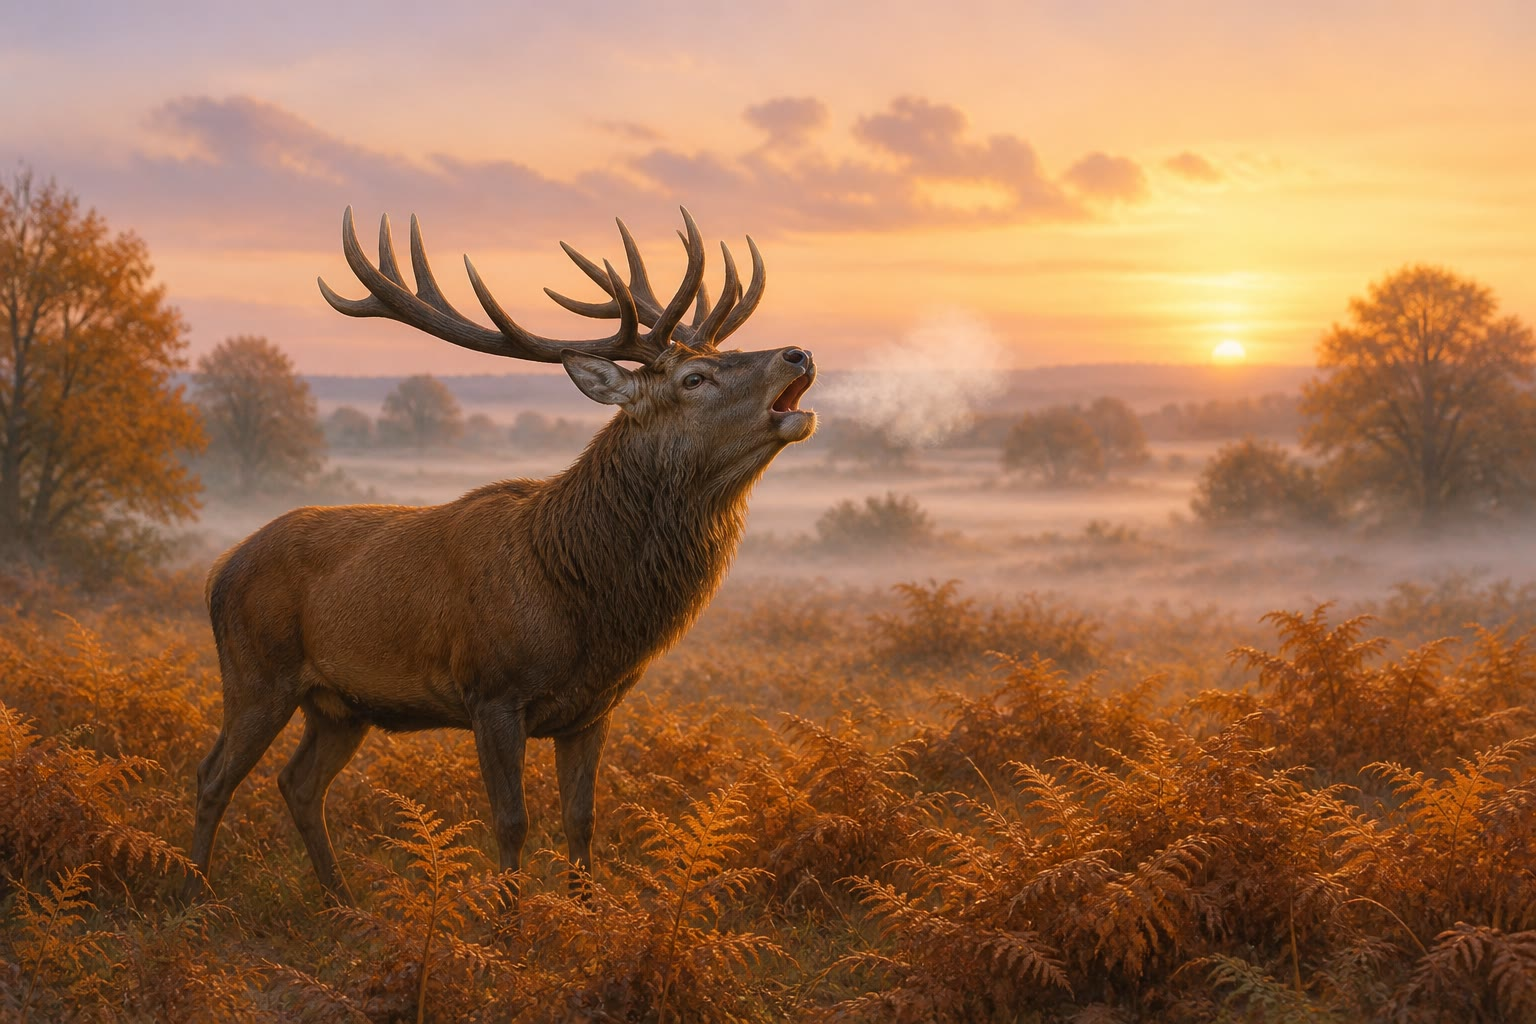
\includegraphics[width=0.6\linewidth]{images/book1/ai/g8-repro-stag.jpg}

{\small 秋日的鸣叫，春日的算术：雄鹿的
时机已把妊娠期算进去。}
\end{omfigure}

\begin{omfigure}
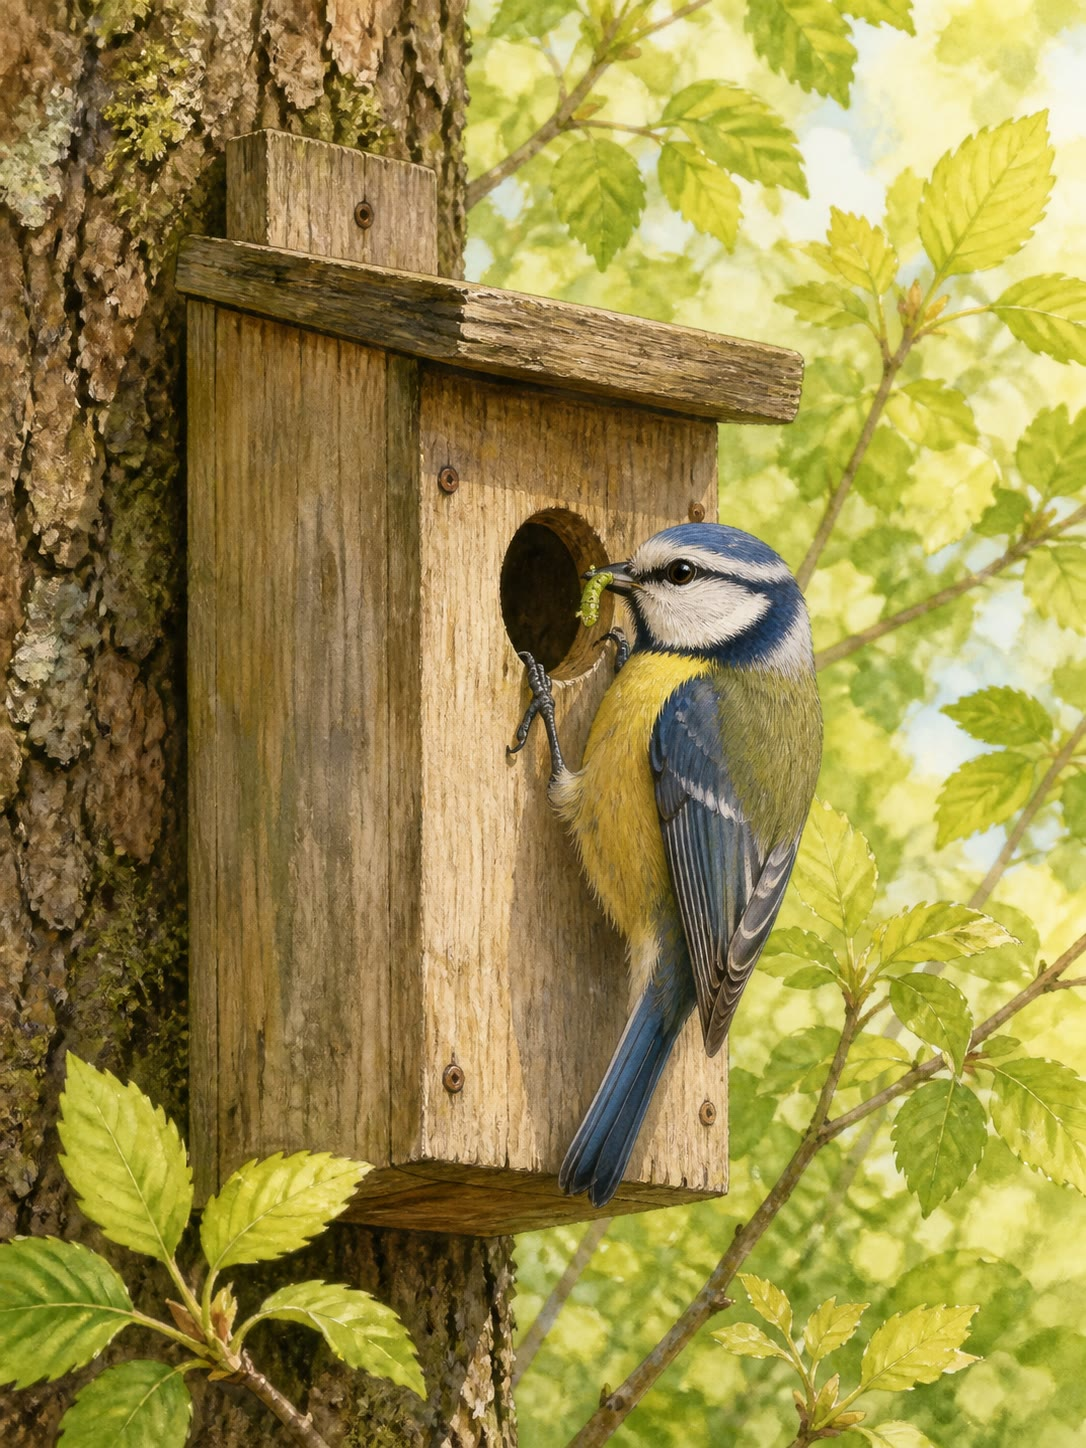
\includegraphics[width=0.46\linewidth]{images/book1/ai/g8-env-nestbox.jpg}

{\small \omterm{def:g2:where-animals-live:habitat}{栖息地}质量的体现：一只蓝山雀和
它的产卵所对应的\omterm{ex:g2:animals-grow-up:butterfly}{毛毛虫}。}
\end{omfigure}

\begin{example}[室内羔羊]\label{ex:g8:reproduction-and-environment:lambs}
绵羊饲养者直接利用这一线索：母羊
在日照\emph{变短}时进入发情状态；若在
先长后短的人工光照下饲养，整群羊
便可提前产羔，以赶上利润丰厚的早期市场。
其机制读取的是光照而非日历——改变光照，
日历也随之而变。线索一旦明确，便成了杠杆。
\end{example}

\section{由栖息地供给}

\begin{proposition}[繁殖需以物质为代价]\label{prop:g8:reproduction-and-environment:cost}
卵、\omterm{def:g2:animals-grow-up:born}{乳汁}、花蜜、\omterm{def:g2:from-seed-to-plant:seed}{种子}和鹿角，都属于
\emph{生产}，即
\cref{def:g6:matter-from-food:production}所指的含义——
即亲代必须先获取的\omterm{def:g6:plants-are-producers:matter}{有机物}。因此，
\omterm{def:g2:where-animals-live:habitat}{栖息地}的丰富程度决定了预算：
\begin{itemize}
  \item 食物充足的母鸡每天产卵；饥饿的母鸡则停止——
        这正是\cref{pb:g6:matter-from-food:1}的账本，
        收支平衡就落在卵这一项上；
  \item 山毛榉只有在良好生长季之后的大量结实“大年”，
        在良好的生长季之后——\omterm{def:g2:from-seed-to-plant:seed}{种子}的收成
        是夏季积累下来的储备
        （见\cref{ex:g6:plants-are-producers:pantry}）；
  \item 艰难的年景会减少产卵数：许多\omterm{prop:g3:sorting-living-things:groups}{鸟类}在猎物稀少时
        产卵减少，甚至不产卵。
\end{itemize}
\end{proposition}
\admitted

\begin{example}[数一数山雀的产卵数]\label{ex:g8:reproduction-and-environment:clutch}
巢箱研究表明，蓝山雀的产卵数随
\omterm{ex:g2:animals-grow-up:butterfly}{毛毛虫}的供应量而变化：橡树林丰富时，产卵十枚或更多；
花园贫瘠时则只有六到七枚。鸟儿并非靠账本决定这一点——
而是靠自身状况，它由\omterm{def:g2:where-animals-live:habitat}{栖息地}的食物建立，
决定了她能够供养多少卵。窝卵数
即\omterm{def:g2:where-animals-live:habitat}{栖息地}质量的写照，写在卵的数目上。
\end{example}

\section{受世界限制：种群}

\begin{definition}[种群]\label{def:g8:reproduction-and-environment:population}
一个\emph{种群}\index{种群}是指
生活在同一地点的同一\omterm{def:g5:biodiversity:species}{物种}的全部个体——例如
池塘中的青蛙、树林中的山毛榉。繁殖使其增加；
死亡和迁出使其减少；\omterm{def:g6:exploring-our-environment:components}{环境}则设定了
上限。
\end{definition}

\begin{proposition}[种群为何不会爆发式增长]\label{prop:g8:reproduction-and-environment:limits}
每个\omterm{def:g5:biodiversity:species}{物种}都过量繁殖——每对青蛙产卵数千，
每棵山毛榉产\omterm{def:g2:from-seed-to-plant:seed}{种子}数千，
（见\cref{prop:g4:animal-reproduction:strategies}），然而
池塘里并没有挤满青蛙。过剩的个体要经受
\omterm{def:g6:exploring-our-environment:components}{环境}的制约：
\begin{itemize}
  \item \emph{捕食}——
        \cref{ex:g4:animal-reproduction:pondcount}中的苍鹭与蜻蜓幼虫；
  \item \emph{食物与空间}——只有这么多的
        \omterm{ex:g2:animals-grow-up:butterfly}{毛毛虫}、巢洞和落在林地上的
        光斑；
  \item \emph{\omterm{def:g6:exploring-our-environment:conditions}{条件}}——花期的晚霜
        （见\cref{exo:g3:flowers-fruits-seeds:9}），干旱使
        \omterm{ex:g2:animals-grow-up:frog}{蝌蚪}的池塘日渐缩小。
\end{itemize}
平均而言，在稳定的\omterm{def:g2:where-animals-live:habitat}{栖息地}中，每对亲本
自身得以替换——
这正是\cref{prop:g5:food-webs:balance}中的平衡，
从亲代的角度来看。
\end{proposition}
\admitted

\begin{example}[池塘边的两个春季]\label{ex:g8:reproduction-and-environment:twosprings}
第一个春季，温和湿润：水位高，\omterm{prop:g3:sorting-living-things:groups}{昆虫}出现早——
卵以数千计，幼蛙以数百计，\omterm{def:g8:reproduction-and-environment:population}{种群}
数量攀升。第二个春季，遭遇干旱：池塘
缩成一洼积水，\omterm{ex:g2:animals-grow-up:frog}{蝌蚪}挤作一团，\omterm{def:g7:what-is-respiration:respiration}{氧气}下降
（\cref{prop:g7:oxygen-in-the-water:drains}），苍鹭
在集中的\omterm{ex:g2:animals-grow-up:frog}{蝌蚪}群中大快朵颐——
仅剩寥寥数只幼蛙。同样的蛙，同样的机制，
两种结局：\omterm{def:g6:exploring-our-environment:components}{环境}每一代都在为之副署。
\end{example}

\begin{remark}[人类改变制约因素]\label{rem:g8:reproduction-and-environment:humans}
人类对野生\omterm{def:g1:animals-around-us:animal}{动物}的多数影响，都通过这些制约因素起作用，
而非通过核心机制：排干的池塘与
连根铲除的树篱，夺走了繁殖\omterm{def:g2:where-animals-live:habitat}{栖息地}
（\cref{prop:g2:where-animals-live:loss}）；杀虫剂
清空了山雀所对准的\omterm{ex:g2:animals-grow-up:butterfly}{毛毛虫}高峰；花园里的
巢箱，以及
\cref{ex:g5:biodiversity:storks}中修复的湿草甸，重新加上了上限。
保护一个\omterm{def:g5:biodiversity:species}{物种}，实际上就是保护
其繁殖所依托的\omterm{def:g6:exploring-our-environment:components}{环境}——线索、
预算与制约因素，须一并保护。
\end{remark}

\begin{method}[审查种群变化]\label{met:g8:reproduction-and-environment:audit}
\omterm{def:g8:reproduction-and-environment:population}{种群}数量升降时，依次审查：
\begin{enumerate}
  \item \emph{时机}：线索与资源高峰是否
        仍然吻合？（春季过早，可能使雏鸟
        孵出时\omterm{ex:g2:animals-grow-up:butterfly}{毛毛虫}已过高峰）；
  \item \emph{预算}：当季\omterm{def:g2:where-animals-live:habitat}{栖息地}使亲代
        能供给多少资源？
  \item \emph{制约}：哪些发生了变化——捕食者、食物、
        空间、\omterm{def:g6:exploring-our-environment:conditions}{条件}？
  \item \emph{\omterm{def:g2:where-animals-live:habitat}{栖息地}}：繁殖场所本身是
        增加还是减少？
\end{enumerate}
\end{method}

\section{练习}

\begin{exercise}[$\star$]\label{exo:g8:reproduction-and-environment:1}
蓝山雀为何在此时产卵？请说出
其所遵循的规律与线索。
\end{exercise}

\begin{exercise}[$\star$]\label{exo:g8:reproduction-and-environment:2}
雄鹿的秋季时机达成了什么效果，
还须计入哪些因素？
\end{exercise}

\begin{exercise}[$\star$]\label{exo:g8:reproduction-and-environment:3}
繁殖为何被称为“以物质支付”？请列出三项
来自
\cref{prop:g8:reproduction-and-environment:cost}中的支付。
\end{exercise}

\begin{exercise}[$\star$]\label{exo:g8:reproduction-and-environment:4}
什么是\omterm{def:g8:reproduction-and-environment:population}{种群}？什么使其增加，什么使其减少，
什么设定了上限？
\end{exercise}

\begin{exercise}[$\star$]\label{exo:g8:reproduction-and-environment:5}
说出消耗蛙类过剩个体的三种制约因素。
\end{exercise}

\begin{exercise}[$\star$]\label{exo:g8:reproduction-and-environment:6}
十枚卵与六枚卵的山雀窝卵数对比说明了什么，
又反映了什么？
\end{exercise}

\begin{exercise}[$\star\star$]\label{exo:g8:reproduction-and-environment:7}
解释养羊者的光照技巧，以及它
证明了关于线索的什么。
\end{exercise}

\begin{exercise}[$\star\star$]\label{exo:g8:reproduction-and-environment:8}
复述\cref{ex:g8:reproduction-and-environment:twosprings}，
以\cref{met:g8:reproduction-and-environment:audit}的四个问题为纲，
针对第二个春季作答。
\end{exercise}

\begin{exercise}[$\star\star$]\label{exo:g8:reproduction-and-environment:9}
气候变暖使橡树\omterm{ex:g2:animals-grow-up:butterfly}{毛毛虫}提前
两周出现，而山雀的日长线索未变。
预测这一错配，并说明它对应审查中的哪一项。
\end{exercise}

\begin{exercise}[$\star\star$]\label{exo:g8:reproduction-and-environment:10}
“鳕鱼的数百万卵并不白费——它们
是被消耗掉的。”请以
\cref{prop:g8:reproduction-and-environment:limits}为依据，为这句话辩护。
\end{exercise}

\begin{exercise}[$\star\star$]\label{exo:g8:reproduction-and-environment:11}
各项人类行为分别改变了哪一项制约：排干
沼泽；挂设巢箱；五月为果园喷药防治
\omterm{ex:g2:animals-grow-up:butterfly}{毛毛虫}；修复湿草甸？
\end{exercise}

\begin{exercise}[$\star\star\star$]\label{exo:g8:reproduction-and-environment:12}
用一段话串联三章：繁殖策略主线
（\cref{prop:g4:animal-reproduction:strategies}）、金字塔的
损耗（\cref{ex:g6:matter-from-food:pyramid}），以及本章
的制约因素，与之合为一套解释，说明为何
池塘并未被蛙类挤得满满当当。
\end{exercise}

\section{问题：巢箱账目}

\begin{problem}[{周末问题——十年蓝山雀，
逐箱审计}]\label{pb:g8:reproduction-and-environment:1}
某学校十年间监测二十个巢箱：
产卵日期、窝卵数、每箱离巢幼鸟数，并与
天气记录和园丁的日记并列记录。

\medskip\noindent\textbf{第一部分——读懂正常
年份。}
\begin{enumerate}
  \item 第 1--4 年：四月下旬产卵，每窝
        八至十枚卵，多数卵孵化后离巢。说出
        决定四月下旬产卵的线索，以及产卵时间
        所对准的高峰。
  \item 第 3 年的窝卵数，在第 2 年温暖、\omterm{ex:g2:animals-grow-up:butterfly}{毛毛虫}丰富的五月之后
        每窝多出一两枚卵，亲鸟越冬
        状况良好。这一相关性所说明的是哪条
        命题？
  \item 即使在好年份，约五分之一的卵
        始终不能离巢。列出可能导致此现象的制约因素，依据
        \cref{prop:g8:reproduction-and-environment:limits}。
  \item 学校为何要将天气与园务工作的记录
        与卵的记录并列？（请用审计的四个
        问题作答。）
\end{enumerate}

\medskip\noindent\textbf{第二部分——异常情况。}
\begin{enumerate}[resume]
  \item 第 5 年：三月异常温暖，\omterm{ex:g2:animals-grow-up:butterfly}{毛毛虫}
        提前两周出现；产卵日期几乎未变。
        预测第 5 年的离巢数，并指出
        失效的审计项。
  \item 第 6 年：园丁日记记载，老橡树的
        枯枝被清除，草地带
        每月割草一次。离巢数下降，
        尽管天气宜人。日记涉及
        哪些审计项？
  \item 第 7 年：一对雀鹰定居。窝卵数
        不变，但幼鸟离巢数下降。哪一项
        制约因素发生了变化，为何\emph{窝卵数}审计项
        没有随之变化？
  \item 第 8 年：巢箱增至四十个；离巢幼鸟总数
        增加，但\emph{每箱}成功率保持稳定。
        新增巢箱提高了哪一个上限，又有哪一项
        未受影响？
\end{enumerate}

\medskip\noindent\textbf{第三部分——报告。}
\begin{enumerate}[resume]
  \item 写出一句十年总结，将
        窝卵数与\omterm{def:g2:where-animals-live:habitat}{栖息地}质量联系起来，并引用
        \cref{ex:g8:reproduction-and-environment:clutch}。
  \item 镇里提议砍伐橡树行，改建停车场，
        并以增设五十个巢箱作“补偿”。
        请审计此方案：在线索、预算、
        制约因素和\omterm{def:g2:where-animals-live:habitat}{栖息地}中，巢箱能替代哪些，又有哪些
        只有橡树才能提供？
  \item 为第 11 年推荐两项园务措施，每项
        均与其对应的审计项相联系。
  \item 用一句话总结本章的道理：
        除双亲外，每只幼鸟还需要
        什么？
\end{enumerate}
\end{problem}
